\PassOptionsToPackage{dvipsnames,svgnames,x11names}{xcolor}
\documentclass[tikz,border=8pt]{standalone}
\usetikzlibrary{arrows.meta,positioning,calc,shapes,shadows,decorations.pathmorphing,shapes.geometric,backgrounds,decorations.markings,decorations.pathreplacing,decorations.text,fit,shapes.misc,shapes.arrows,matrix,bending,3d,chains,intersections,shapes.symbols,svg.path,shapes.multipart,snakes,shapes.callouts,angles,quotes}
\usepackage{amsmath}
\usepackage{amssymb}
\usepackage{fontawesome5}
\usetikzlibrary{fadings,shadows.blur,patterns,patterns.meta}

\providecolor{gold}{RGB}{212,175,55}
\providecolor{silver}{RGB}{192,192,192}
\providecolor{bronze}{RGB}{205,127,50}
\providecolor{darkblue}{RGB}{0,0,139}
\providecolor{lightblue}{RGB}{173,216,230}
\providecolor{darkgreen}{RGB}{0,100,0}
\providecolor{lightgreen}{RGB}{144,238,144}
\providecolor{darkred}{RGB}{139,0,0}
\providecolor{navy}{RGB}{0,0,128}
\providecolor{skyblue}{RGB}{135,206,235}
\providecolor{beige}{RGB}{245,245,220}
\providecolor{cream}{RGB}{255,253,208}

% --- DEFINE CUSTOM COLORS (Curated High-End Tech Palette) ---
\definecolor{imgcol}{RGB}{30, 115, 190}    % Deep Sapphire Blue
\definecolor{boxcol}{RGB}{225, 50, 50}     % Vibrant Crimson
\definecolor{mathcol}{RGB}{142, 68, 173}   % Rich Amethyst Purple
\definecolor{textdark}{RGB}{33, 43, 54}    % Deep Charcoal / Navy

\begin{document}
\begin{tikzpicture}[
    font=\sffamily,
    >={Stealth[scale=1.2]},
    panel/.style={
        fill=white,
        draw=gray!30,
        rounded corners=8pt,
        inner sep=12pt,
        text width=8.5cm,
        minimum height=3.5cm,
        align=left,
        blur shadow={shadow opacity=15, shadow yshift=-2pt, shadow xshift=2pt}
    },
    rulerline/.style={ultra thick, -Stealth}
]

% --- ABSOLUTE BACKGROUND & GRID ---
\fill[white] (-8, -2) rectangle (33.0695,22.3329);
\draw[step=1cm, gray!15, very thin] (-8, -2) grid (33.0695,22.3329);

% --- TITLE BOX ---
\node[align=center, fill=white, inner sep=10pt, anchor=center] at (9.1005,20.2003) {
    {\bfseries\Huge\color{textdark} Algorithmic Pinning via \texttt{object-position}}\\[6pt]
    {\large\color{gray} Mapping internal coordinate offsets to lock a focus point (\texttt{object-position: 50\% 20\%})}
};


% ==========================================
% ZONE 1: THE VISUAL DIAGRAM (LEFT SIDE)
% ==========================================

% 1. The Scaled Image (Background & Boundary)
\fill[imgcol!10] (2, 0) rectangle (10, 16);
\draw[step=1cm, imgcol!25, thin] (2, 0) grid (10, 16);

% Vector Silhouette Avatar (Mathematically Perfect Geometric Primitives)
\begin{scope}
    \clip (2, 0) rectangle (10, 16);
    % Body
    \path[fill=textdark!80] (2.5, 0) -- (2.5, 6) .. controls (2.5, 9.5) and (4.5, 9.5) .. (5, 9.5) -- (7, 9.5) .. controls (7.5, 9.5) and (9.5, 9.5) .. (9.5, 6) -- (9.5, 0) -- cycle;
    % Neck
    \fill[textdark!70] (5.2, 9) rectangle (6.8, 11.5);
    % Head (The Mathematical Lock at X=6, Y=12.8)
    \fill[textdark!85] (6, 12.8) ellipse (1.6 and 2.1);
\end{scope}

\draw[imgcol, ultra thick] (2, 0) rectangle (10, 16);

% Image Focal Target Line & Label (Moved to empty left side)
\draw[imgcol, ultra thick, dashed] (1.5, 12.8) -- (10.5, 12.8);
\node[anchor=south east, imgcol, font=\bfseries, fill=white, inner sep=2pt] at (-0.5, 13.0) {Image 20\% Focal Line};

% DSLR-Style Camera Focal Target Reticle
\draw[thick, boxcol] (5.5, 13.3) -- (5.5, 13.5) -- (5.7, 13.5); % Top-left bracket
\draw[thick, boxcol] (6.5, 13.3) -- (6.5, 13.5) -- (6.3, 13.5); % Top-right bracket
\draw[thick, boxcol] (5.5, 12.3) -- (5.5, 12.1) -- (5.7, 12.1); % Bottom-left bracket
\draw[thick, boxcol] (6.5, 12.3) -- (6.5, 12.1) -- (6.3, 12.1); % Bottom-right bracket
\draw[boxcol, thick] (6, 12.8) circle (0.35);
\draw[boxcol, thick] (5.3, 12.8) -- (5.7, 12.8);
\draw[boxcol, thick] (6.3, 12.8) -- (6.7, 12.8);
\draw[boxcol, thick] (6, 12.1) -- (6, 12.5);
\draw[boxcol, thick] (6, 13.1) -- (6, 13.5);
\fill[boxcol] (6, 12.8) circle (0.05);

% 2. Crop Shading (Web Inspector Style Structural Hash + 75% White Fill)
\fill[pattern={Lines[angle=45,distance={5pt},line width=0.6pt]}, pattern color=gray!40] (2, 0) rectangle (10, 9.6);
\fill[white, opacity=0.75] (2, 0) rectangle (10, 9.6);

\fill[pattern={Lines[angle=45,distance={5pt},line width=0.6pt]}, pattern color=gray!40] (2, 13.6) rectangle (10, 16);
\fill[white, opacity=0.75] (2, 13.6) rectangle (10, 16);

% 3. The Viewport Boundary
\draw[boxcol, ultra thick, dashed] (2, 9.6) rectangle (10, 13.6);

% 4. Browser Chrome Bar
\fill[fill=gray!15, draw=boxcol, thick, rounded corners=2pt] (2, 13.6) rectangle (10, 14.1);
\fill[red!80!black] (2.35, 13.85) circle (0.09);
\fill[yellow!80!black] (2.65, 13.85) circle (0.09);
\fill[green!70!black] (2.95, 13.85) circle (0.09);
\node[font=\scriptsize\ttfamily\bfseries, textdark] at (6, 13.85) {viewport: 800px $\times$ 400px};

% 5. Overlay Labels (Repositioned to Eliminate Collisions)
\node[font=\Large\bfseries, textdark, fill=white, draw=gray!30, inner sep=4pt, rounded corners=2pt, text opacity=1, fill opacity=0.95, anchor=east] at (-0.5, 14.8) {Cropped (Top 240px)};
\draw[-Stealth, thick, textdark] (-0.5, 14.8) -- (2.0, 14.8);

\node[font=\Large\bfseries, textdark, fill=white, draw=gray!30, inner sep=6pt, rounded corners=2pt, text opacity=1, fill opacity=1, anchor=east] at (-0.5, 4.8) {Cropped (Bottom 960px)};
\draw[-Stealth, thick, textdark] (-0.5, 4.8) -- (2.0, 4.8);

% "Visible Container Area" Label with Pointer Arrow
\node[font=\Large\bfseries, boxcol, fill=white, draw=gray!30, inner sep=4pt, rounded corners=2pt, text opacity=1, fill opacity=0.95, anchor=east] (vislabel) at (-0.5, 11.6) {Visible Container Area};
\draw[-Stealth, thick, boxcol] (-0.5, 11.6) -- (2.0, 11.6);


% ==========================================
% ZONE 2: THE AXES & MEASUREMENT SCALES
% ==========================================

% Left Axis (Image Pixel Ruler - Blue, Relocated to X = -6.0)
\draw[rulerline, imgcol] (-6.0, 16) -- (-6.0, 0);
\foreach \y in {0,1,...,16} {
    \draw[imgcol!60, thin] (-6.1, \y) -- (-5.9, \y);
}
\draw[imgcol, ultra thick] (-6.3, 16) -- (-5.7, 16);
\node[anchor=east, font=\bfseries, textdark, fill=white, inner sep=3pt] at (-6.3, 16) {0px (0\%)};
\draw[imgcol, ultra thick] (-6.3, 12.8) -- (-5.7, 12.8);
\node[anchor=east, font=\bfseries, imgcol, fill=white, inner sep=3pt] at (-6.3, 12.8) {320px (20\%)};
\draw[imgcol, ultra thick] (-6.3, 0) -- (-5.7, 0);
\node[anchor=east, font=\bfseries, textdark, fill=white, inner sep=3pt] at (-6.3, 0) {1600px (100\%)};

% Right Axis (Container Pixel Ruler - Red, Relocated to X = 11.5)
\draw[rulerline, boxcol] (11.5, 13.6) -- (11.5, 9.6);
\foreach \y in {9.6, 10.6, 11.6, 12.6, 13.6} {
    \draw[boxcol!60, thin] (11.4, \y) -- (11.6, \y);
}
\draw[boxcol, ultra thick] (11.4, 13.6) -- (11.6, 13.6);
\node[anchor=west, font=\bfseries, textdark, fill=white, inner sep=3pt] at (11.7, 13.6) {0px (0\%)};
\draw[boxcol, ultra thick] (11.4, 12.8) -- (11.6, 12.8);
\node[anchor=west, font=\bfseries, boxcol, fill=white, inner sep=3pt] at (11.7, 12.8) {80px (20\%)};
\draw[boxcol, ultra thick] (11.4, 9.6) -- (11.6, 9.6);
\node[anchor=west, font=\bfseries, textdark, fill=white, inner sep=3pt] at (11.7, 9.6) {400px (100\%)};


% ==========================================
% ZONE 3: BRIDGING ANNOTATIONS (THE MIDDLE)
% ==========================================

% Translation Shift Visualizer (Purple Arrow at X = 14.5)
\draw[-Stealth, ultra thick, mathcol] (14.5, 13.6) -- (14.5, 16);
\draw[gray, thick, dotted] (10, 16) -- (14.5, 16);
\draw[gray, thick, dotted] (10, 13.6) -- (11.3, 13.6);
\draw[gray, thick, dotted] (13.6, 13.6) -- (14.5, 13.6);
\node[anchor=west, mathcol, font=\Large\bfseries, fill=white, inner sep=2pt, text width=6cm] at (15.0, 14.8) {Algorithmic Shift $Y = -240$px};

% The Universal Intersection Line & Algorithmic Pin
\draw[mathcol, ultra thick, dotted] (-6.0, 12.8) -- (11.3, 12.8);
\draw[mathcol, ultra thick, dotted] (13.6, 12.8) -- (14.5, 12.8);
\node[anchor=west, mathcol, font=\large\bfseries, fill=white, inner sep=4pt, text width=7cm, align=left] at (15.0, 12.8) {\faMapPin \ The Algorithmic Pin:\\[3pt] Image 20\% $\equiv$ Container 20\%};


% ==========================================
% ZONE 4: THE MATHEMATICS PANELS (RIGHT SIDE)
% ==========================================

% Panel 1: Geometry (Centered at X = 27.5, Y = 18.5)
\node[panel] at (27.1525,17.145) {
    \textbf{\Large \faExpand \ 1. Dimensions After \texttt{cover}}\\[5pt]
    The browser scales a portrait image to cover a landscape container, preserving aspect ratio:\\[3pt]
    $\bullet$ Container Height ($H_c$): \textbf{400px}\\
    $\bullet$ Scaled Image Height ($H_i$): \textbf{1600px}\\[3pt]
    \textit{This size disparity creates a massive \textbf{1200px} structural overflow on the Y-axis.}
};

% Panel 2: The 20% Calculation (Centered at X = 27.5, Y = 13.5)
\node[panel] at (27.1525,12.145) {
    \textbf{\Large \faCrosshairs \ 2. Identifying 20\% Marks}\\[5pt]
    The \texttt{20\%} value in CSS commands the engine to find the 20\% Y-coordinate in both local spaces:\\[3pt]
    $\bullet$ \textbf{Image:} $1600\text{px} \times 0.20 = \textbf{320px}$\\
    $\bullet$ \textbf{Container:} $400\text{px} \times 0.20 = \textbf{80px}$\\[3pt]
    \textit{Goal: Translate the image so its internal 320px focal mark physically aligns with the container's 80px mark.}
};

% Panel 3: The CSS Rendering Formula (Centered at X = 27.5, Y = 8.5)
\node[panel] at (27.1525,7.145) {
    \textbf{\Large \faCalculator \ 3. The Shift Formula}\\[5pt]
    The absolute physical translation is algebraically calculated by subtracting the focal differences:\\[3pt]
    $\text{Offset}_Y = (H_c - H_i) \times \text{Position}_Y\%$\\
    $\text{Offset}_Y = (400 - 1600) \times 0.20$\\
    $\text{Offset}_Y = -1200 \times 0.20 = \textbf{-240px}$\\[3pt]
    The CSS rendering engine shifts the image origin \textbf{240px UPWARDS}.
};

% Panel 4: The X-Axis (Centered at X = 27.5, Y = 3.5)
\node[panel] at (27.1525,2.145) {
    \textbf{\Large \faArrowsAltH \ 4. What about the 50\% X-Axis?}\\[5pt]
    Since the image width perfectly matches the container width after scaling ($W_c = W_i = 800\text{px}$):\\[3pt]
    $\text{Offset}_X = (800 - 800) \times 0.50$\\
    $\text{Offset}_X = \textbf{0px}$\\[3pt]
    No horizontal shift occurs; the face remains mathematically locked in the absolute center horizontally.
};

\end{tikzpicture}
\end{document}
